\section{Role Based Access Control Standard} \label{sec:core-rbac}

Since the basis for our review is extensions to the core model, we will describe the core model, associated entities and other terminology encountered across the space of our review.  The NIST RBAC model proposed by Ferraiolo et al. \cite{ferraiolokuhn} and later adopted as the official standard for RBAC by the International Committee for Information Technology Standards (INCITS) consists of four basic entities:

\begin{itemize}
\setlength{\itemsep}{0.25pt}
\item a set of \emph{Users}: A user can be a person or an agent.
\item a set of \emph{Roles}: A role is a collection of permissions to perform a specific job function in an organization.
\item a set of \emph{Permissions}: A permission refers to an access mode that can be exercised on an object in the system and a session relates a user to possibly many roles.
\item a set of \emph{Sessions}: In each session, a user can be assigned to some of the roles, only when the corresponding role is enabled for activation for that time.		
\end{itemize}

In RBAC, a user can exercise a permission only if the user is assigned to a role.
In addition to the four basic components, two functions are defined:
the user role assignment (UA) and the role
permission assignment (PA) functions.
UA models assignment of users to roles.
PA models assignment of permissions to roles.

\begin{figure}[ht]
    \centering
        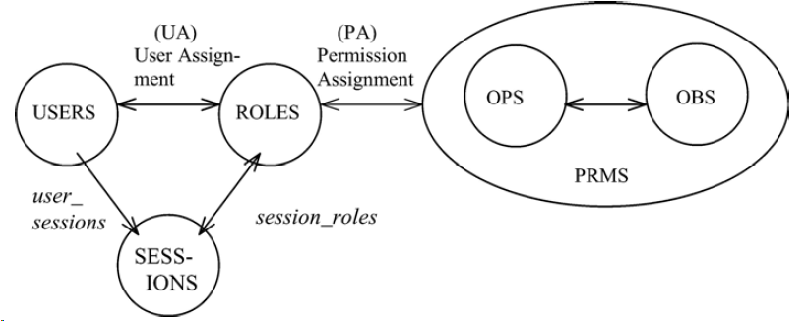
\includegraphics[width=4.0in]{sections/core-model.png}
    \caption{\label{fig:overview}RBAC Core Diagram in NIST RBAC model \cite{ferraiolokuhn}.}
\end{figure}

Figure~\ref{fig:overview} presents an overview of core RBAC model diagram where elements and their relations are described.
Let "USERS", "ROLES", "OBS", "OPS", "PRM", and "SESSIONS" denote users, roles, objects, operations, permissions, and sessions, respectively.
Permissions are associated with possible users' pre-defined operation on an object (e.g., execute a file).
Note that, at user or role activation, a session associated with user or role is established.
